\chapter{Convertidores CC-CC}
\label{convertidores-cc-cc}

\section{Introducción}

Los convertidores electrónicos de potencia de CC-CC actúan como puentes de transferencia de energía entre fuentes y cargas, ambas de corriente continua, que no son compatibles. Un ejemplo es cuando una fuente disponible proporciona una tensión distinta a la requerida por la carga a utilizar. Por eso mismo, la función de estos tipos de  convertidores es la de adaptar tal tensión de la fuente con la máxima eficiencia posible de transferencia de energía.

Normalmente, además de la conversión de nivel de tensión de continua, los convertidores proveen una salida regulada. Dependiendo de la topología del convertidor, la tensión de salida puede ser mayor o menor a la de la entrada.

Los convertidores electrónicos de potencia pueden dividirse en lineales y conmutados. En este capítulo, se presentan los convertidores conmutados, específicamente el convertidor elevador, el cual es utilizado en este trabajo.

\section{Convertidores CC-CC conmutados}

Los convertidores conmutados son una alternativa eficiente respecto de los reguladores lineales. En un circuito de un convertidor conmutado, los transistores operan como llaves, estando completamente prendidos o completamente apagados. Asumiendo que la llave es ideal en la Figura \ref{convertidor-basico}, la salida es igual que la entrada cuando la llave está cerrada, y nula cuando la llave está abierta.

\begin{figure}[hbt!]
    \centering
    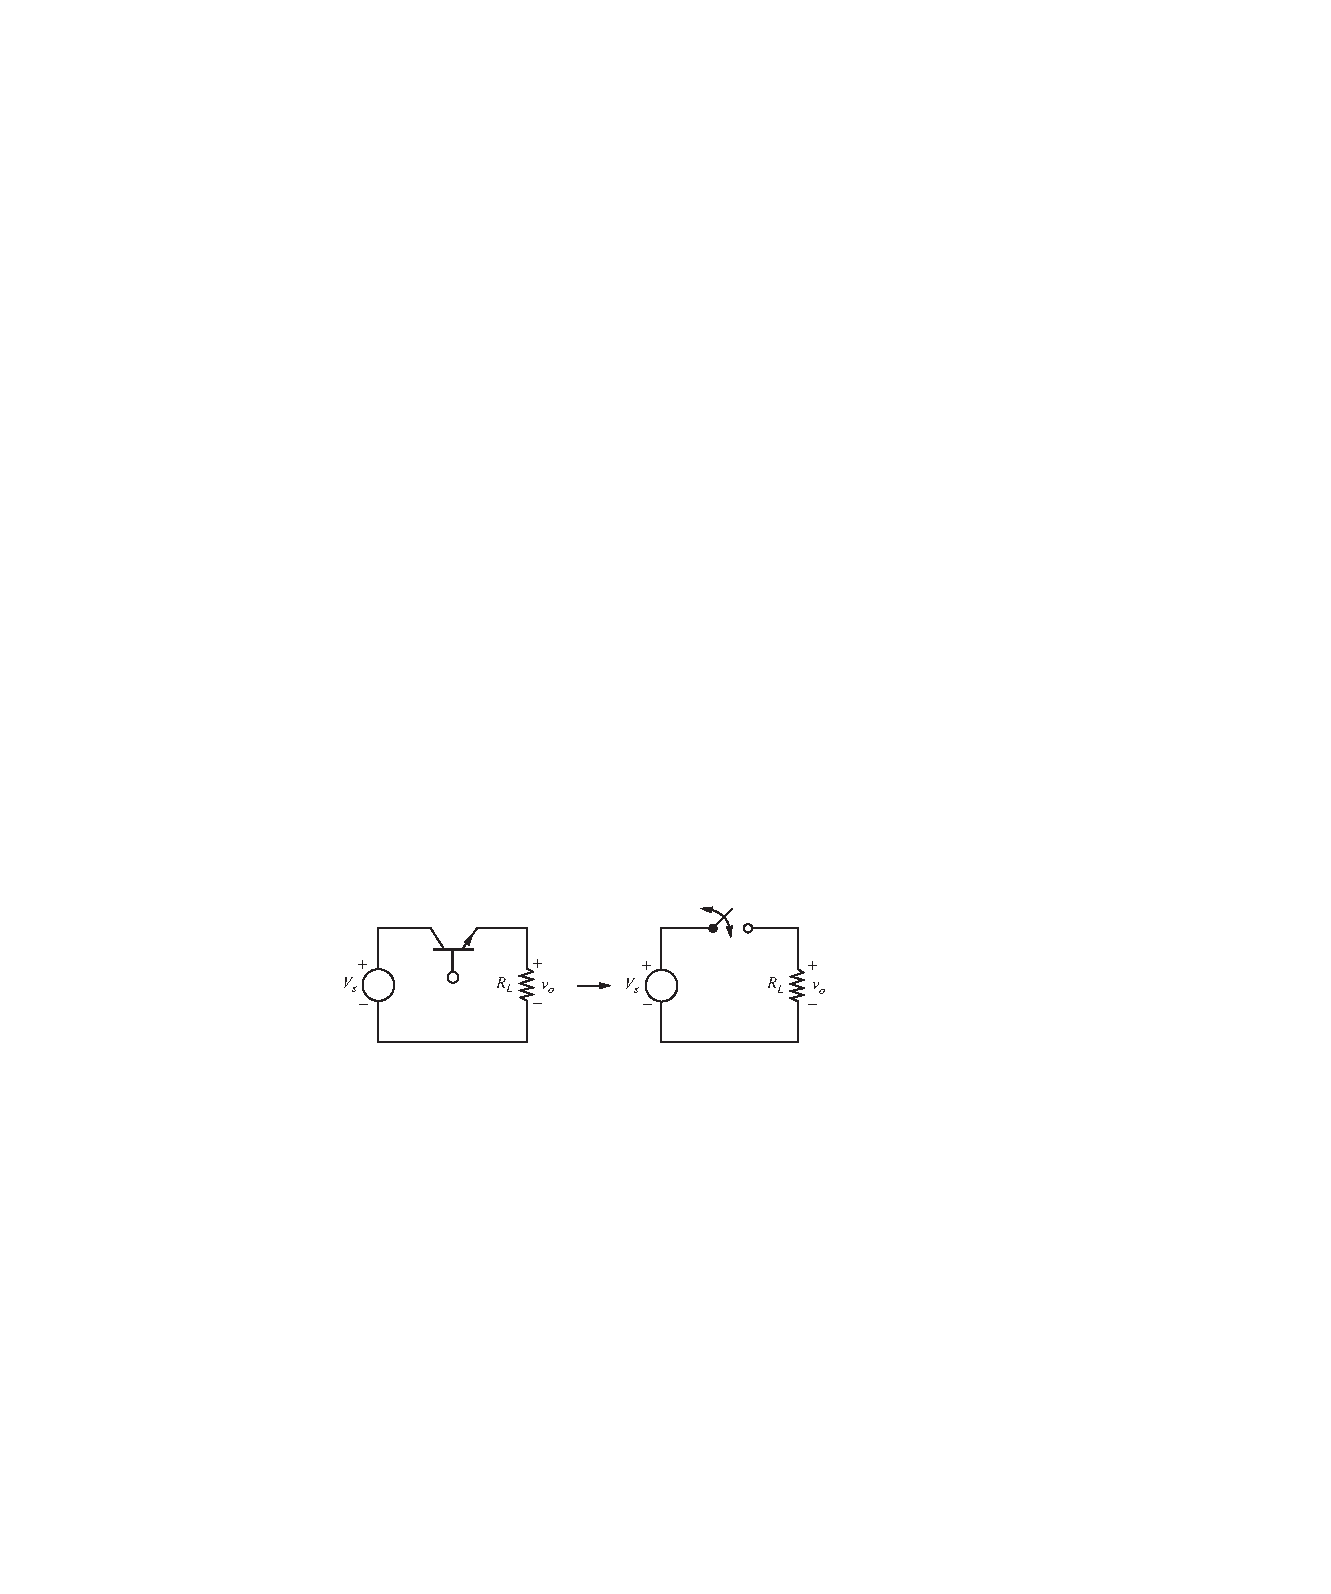
\includegraphics[width=0.55\columnwidth]{Imágenes/Convertidor conmutado básico.pdf}
    \caption{Un convertidor conmutado CC-CC básico y su equivalente de conmutación.}
    \label{convertidor-basico}
\end{figure} 

La conmutación periódica de la llave resulta en la salida en pulsos mostrada en la Figura \ref{salida-conmutador}.

\begin{figure}[hbt!]
    \centering
    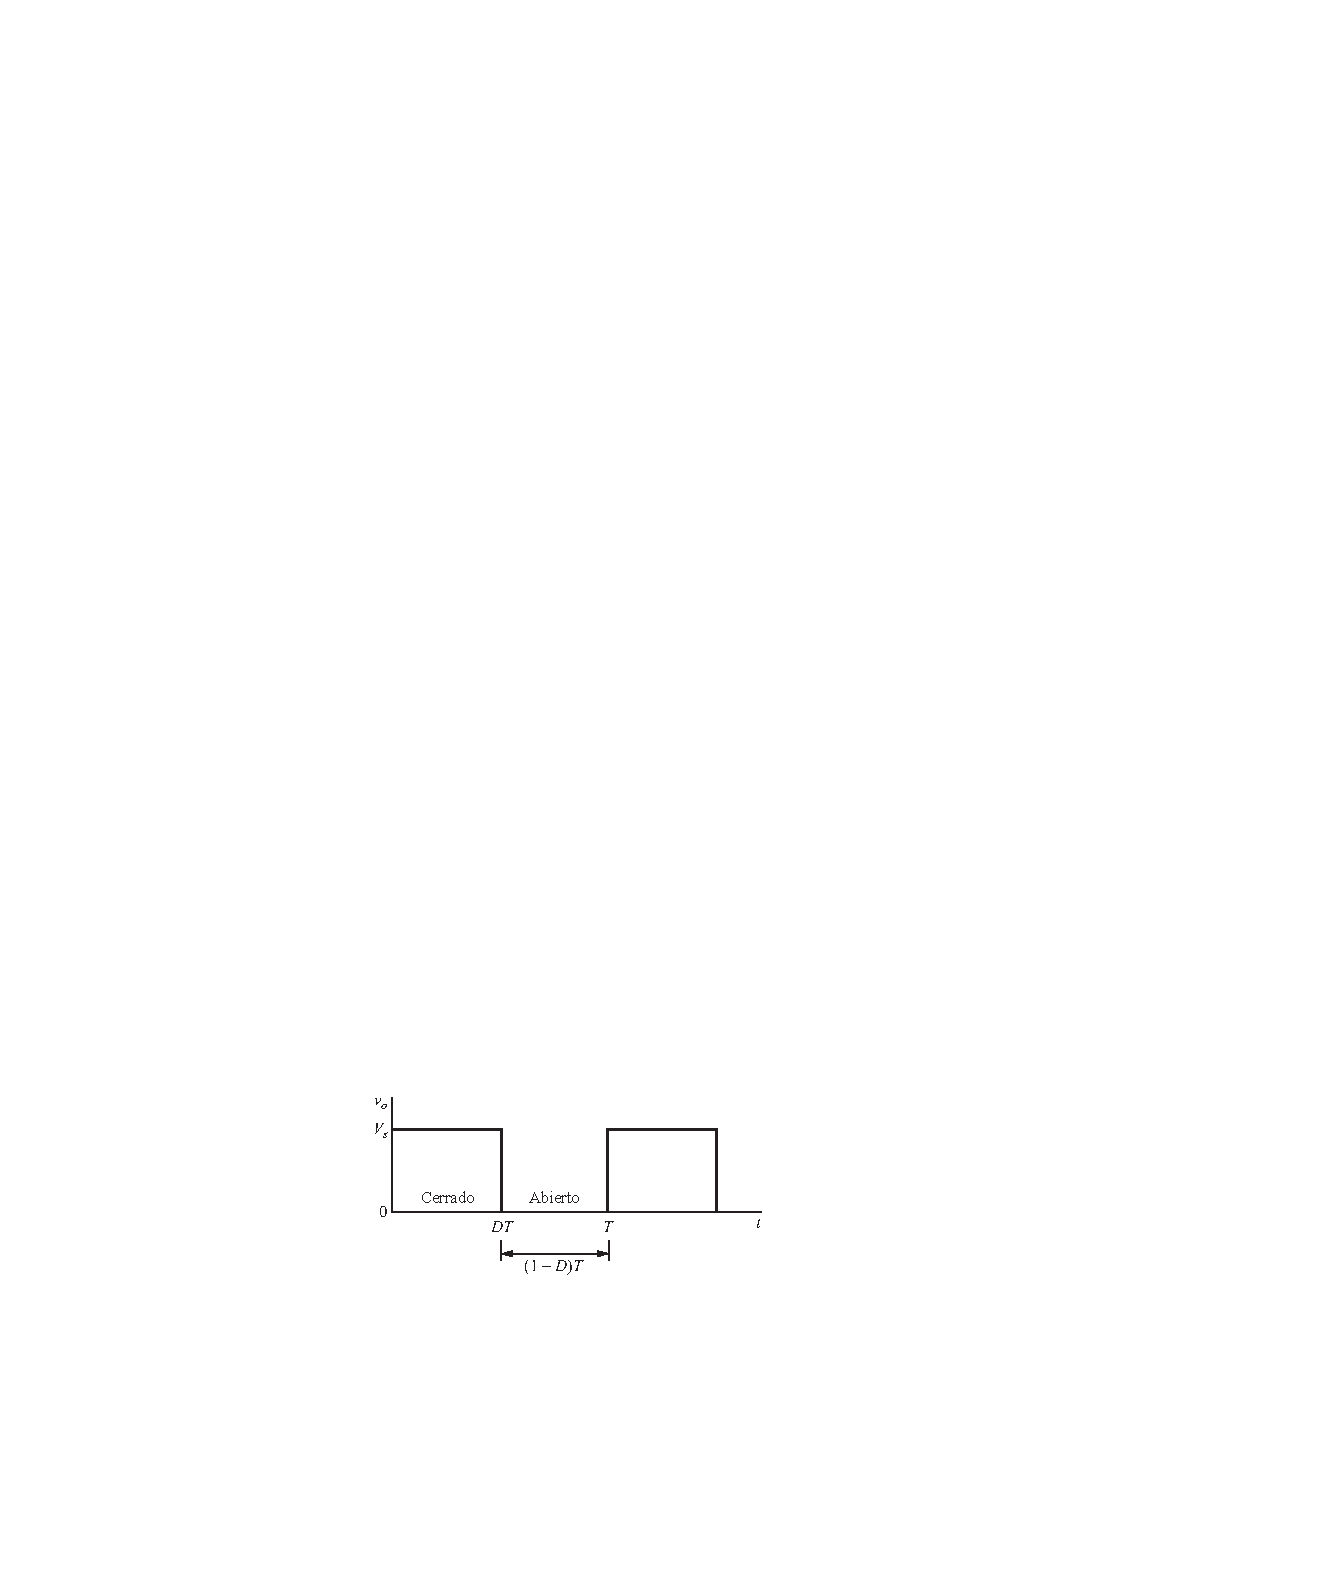
\includegraphics[width=0.55\columnwidth]{Imágenes/Salida del convertidor conmutado básico.pdf}
    \caption{Tensión de salida del circuito de la Figura \ref{convertidor-basico}.}
    \label{salida-conmutador}
\end{figure}

El valor medio de la tensión de salida es:

\begin{equation}   
    V_o = \frac{1}{T} \int_{0}^{T} v_0(t) \,dt = \frac{1}{T} \int_{0}^{DT} V_s \,dt = V_s \, D
\end{equation}

La componente de continua de la tensión de salida es controlada a través del ajuste del tiempo que la llave se encuentra cerrada respecto del período de conmutación total. Esta fracción de tiempo es llamada \emph{ciclo de trabajo} y se representa con la letra $D$.

\begin{equation}
    D \equiv \frac{t_{\mathrm{on}}}{t_{\mathrm{on}} + t_{\mathrm{off}}} = \frac{t_{\mathrm{on}}}{T} = t_{\mathrm{on}} \, f
\end{equation}

En donde $f$ es la frecuencia de conmutación. En este circuito elemental, la componente de continua de la tensión de salida siempre será menor o igual que la tensión de entrada del circuito.

Idealmente, la potencia absorbida por la llave es cero. Cuando la llave está abierta, no circula corriente por ella; cuando está cerrada, no cae tensión. Por lo tanto, toda la potencia es absorbida por la carga, y la eficiencia es del cien por ciento. Con una llave real, las pérdidas son inevitables, ya que ocurre una caída de tensión cuando está cerrada, y debe pasar por la región lineal cuando realiza la conmutación de un estado a otro.

\section{Convertidor elevador}

El convertidor elevador (\emph{boost converter} en inglés) es mostrado en la Figura \ref{convertidor-elevador}. Es llamado de tal manera ya que la tensión de salida es mayor o igual que la de entrada. Este tipo de convertidor es el utilizado para el proyecto, ya que es necesario elevar la tensión del banco de supercapacitores y las baterías de litio.

\begin{figure}[hbt!]
    \centering
    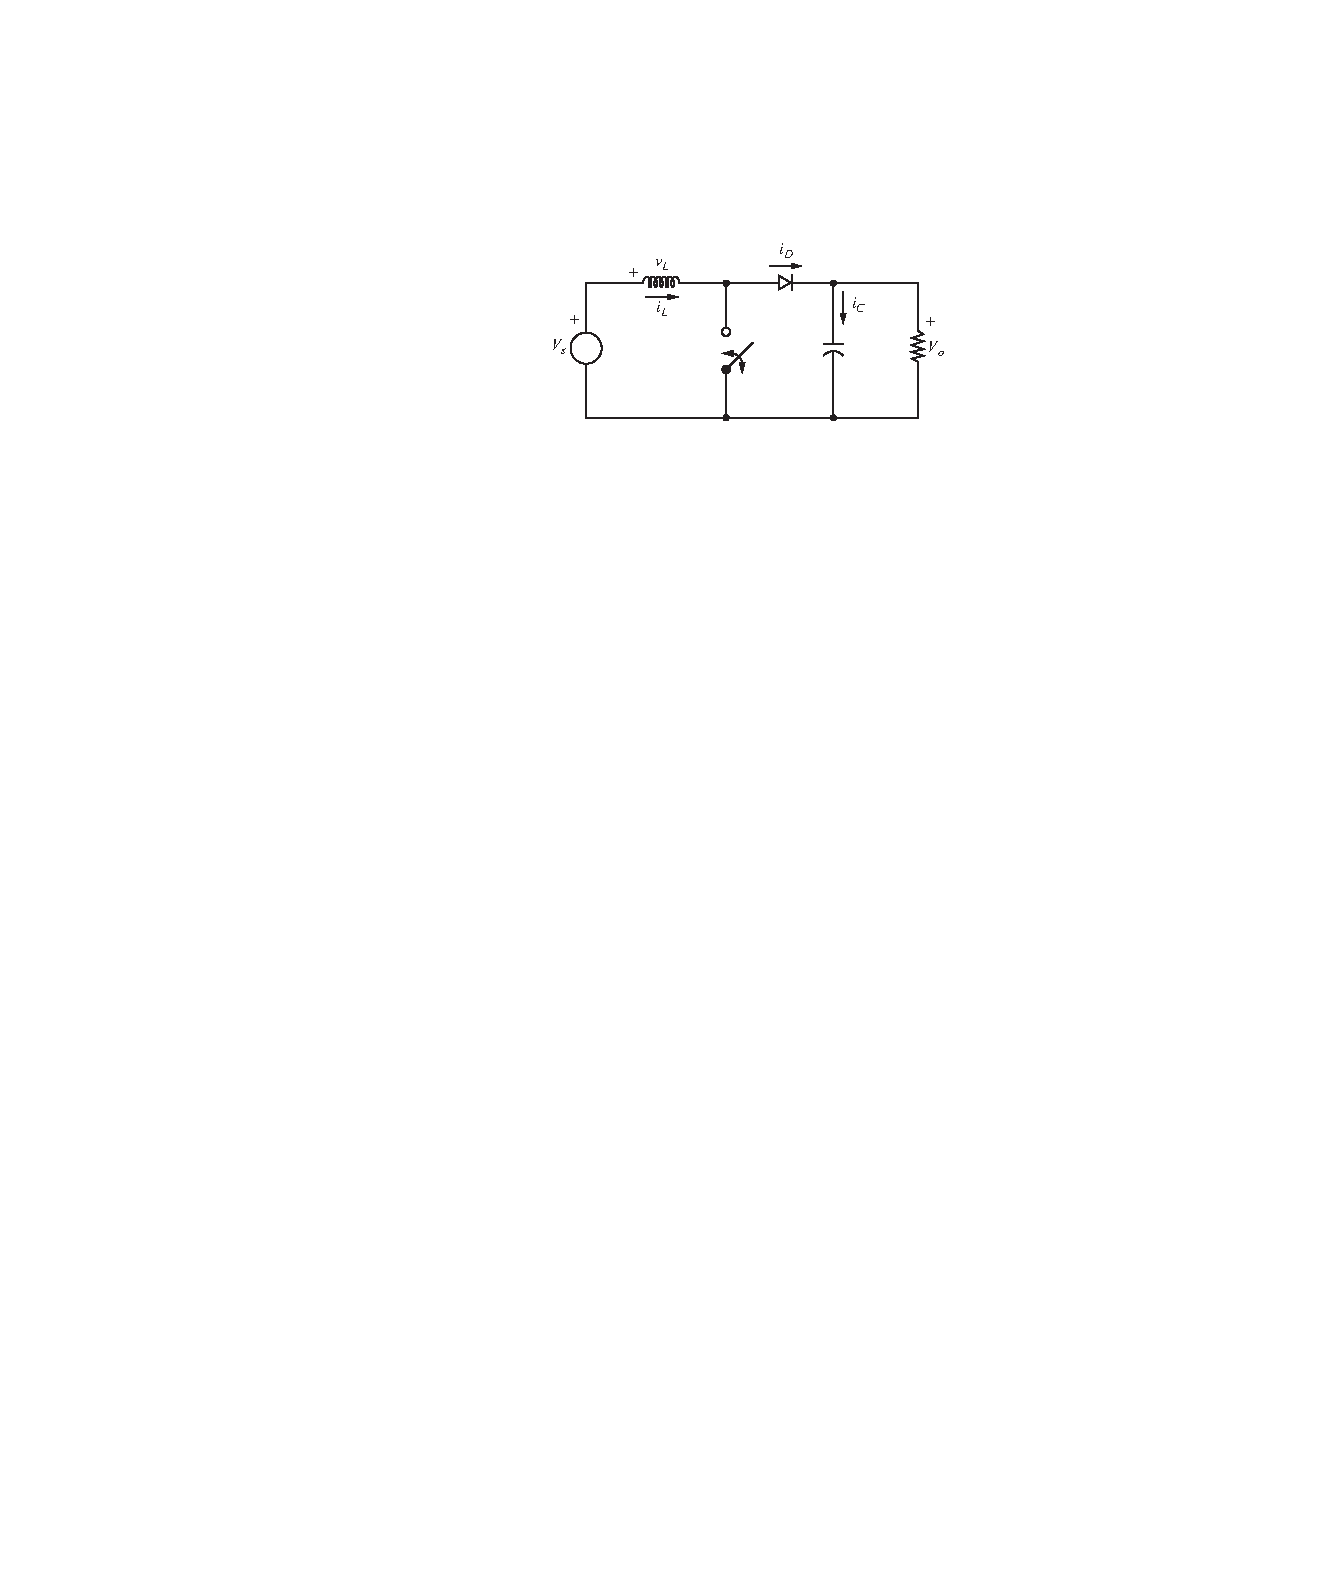
\includegraphics[width=0.55\columnwidth]{Imágenes/Convertidor elevador.pdf}
    \caption{Convertidor elevador.}
    \label{convertidor-elevador}
\end{figure}

Antes de proceder con el análisis de los modos de conducción del convertidor elevador, es necesario realizar las siguientes suposiciones:

\begin{enumerate}
    \item Existen condiciones de estado estacionario.
    \item El período de conmutación es $T$, y la llave está cerrada por un tiempo $DT$ y abierta por un tiempo $(1-D)T$.
    \item La corriente por el inductor es continua (y siempre positiva).
    \item El capacitor posee una capacitancia muy grande, y la tensión de salida es mantenida constante a un valor $V_o$.
    \item Los componentes son ideales.
\end{enumerate}

\subsection{Modo de conducción continua}

Este análisis es hecho a través de la examinación de la tensión y corriente del inductor cuando la llave está cerrada, y nuevamente cuando la llave se encuentra abierta.

\subsubsection{Análisis con la llave cerrada}

Cuando la llave se encuentra cerrada, el diodo se encuentra polarizado inversamente. La ley de Kirchhoff sobre el camino que contiene la fuente, el inductor, y la llave es:
 
\begin{equation}
    v_L = V_s = L \frac{di_L}{dt} \hspace{0.6cm} \textrm{ó} \hspace{0.6cm} \frac{di_L}{dt} = \frac{V_s}{L}
\end{equation}

La derivada de la corriente es una constante, lo que significa que la corriente incrementa linealmente cuando la llave está cerrada, como se muestra en la Figura \ref{formas-onda-elevador}b. Por lo tanto, resolviendo para la tasa de cambio de la corriente del inductor $\Delta i_L$ resulta en:

\begin{equation}
    \boxed{(\Delta i_L)_{\mathrm{cerrada}} = \frac{V_s \, D \, T}{L}}
    \label{llave-cerrada}
\end{equation}

\begin{figure}[hbt!]
    \centering
    \subfloat[Tensión en el inductor.]{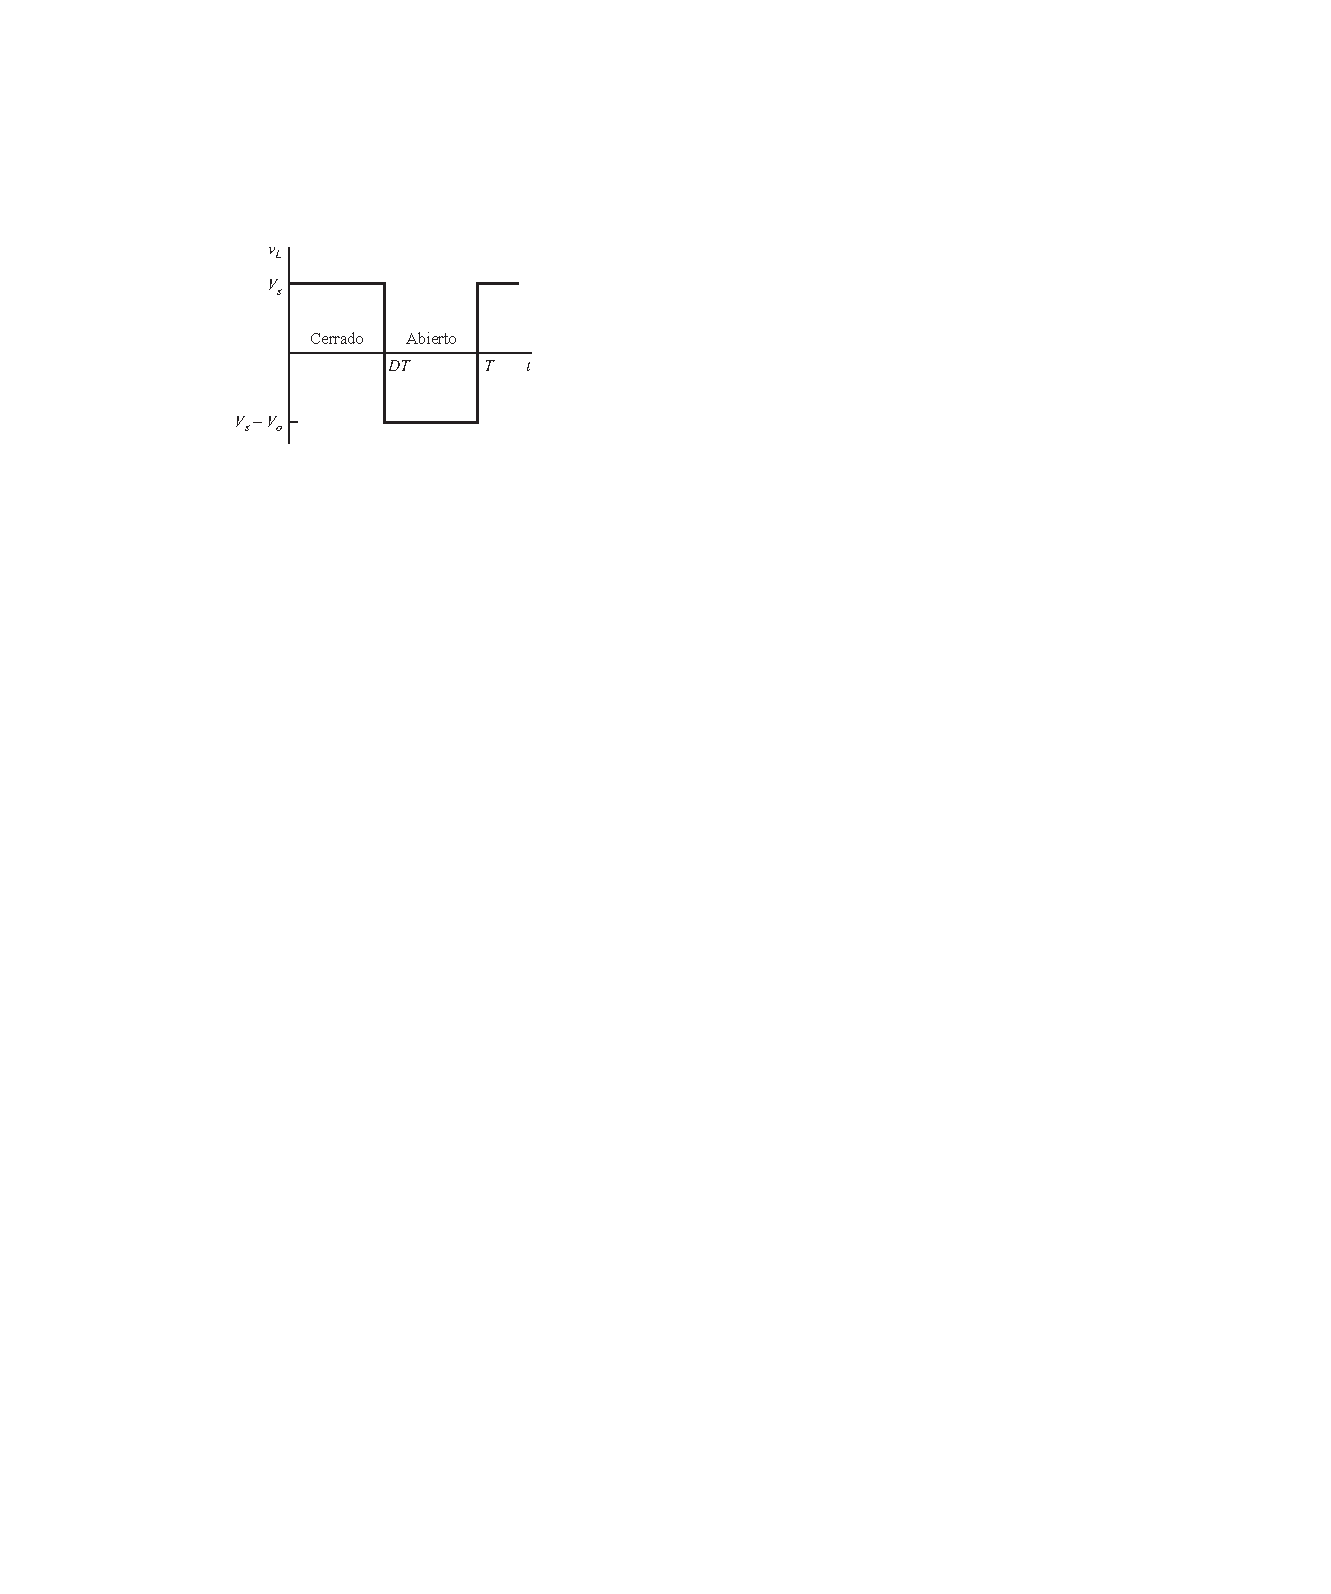
\includegraphics[width=0.38\textwidth]{Imágenes/Convertidor elevador/Tensión del inductor.pdf}}    
    \hspace{10mm}
    \subfloat[Corriente por el inductor.]{\includegraphics[width=0.38\textwidth]{Imágenes/Convertidor elevador/Corriente del inductor.pdf}}
    \hspace{10mm}
    \subfloat[Corriente por el diodo]{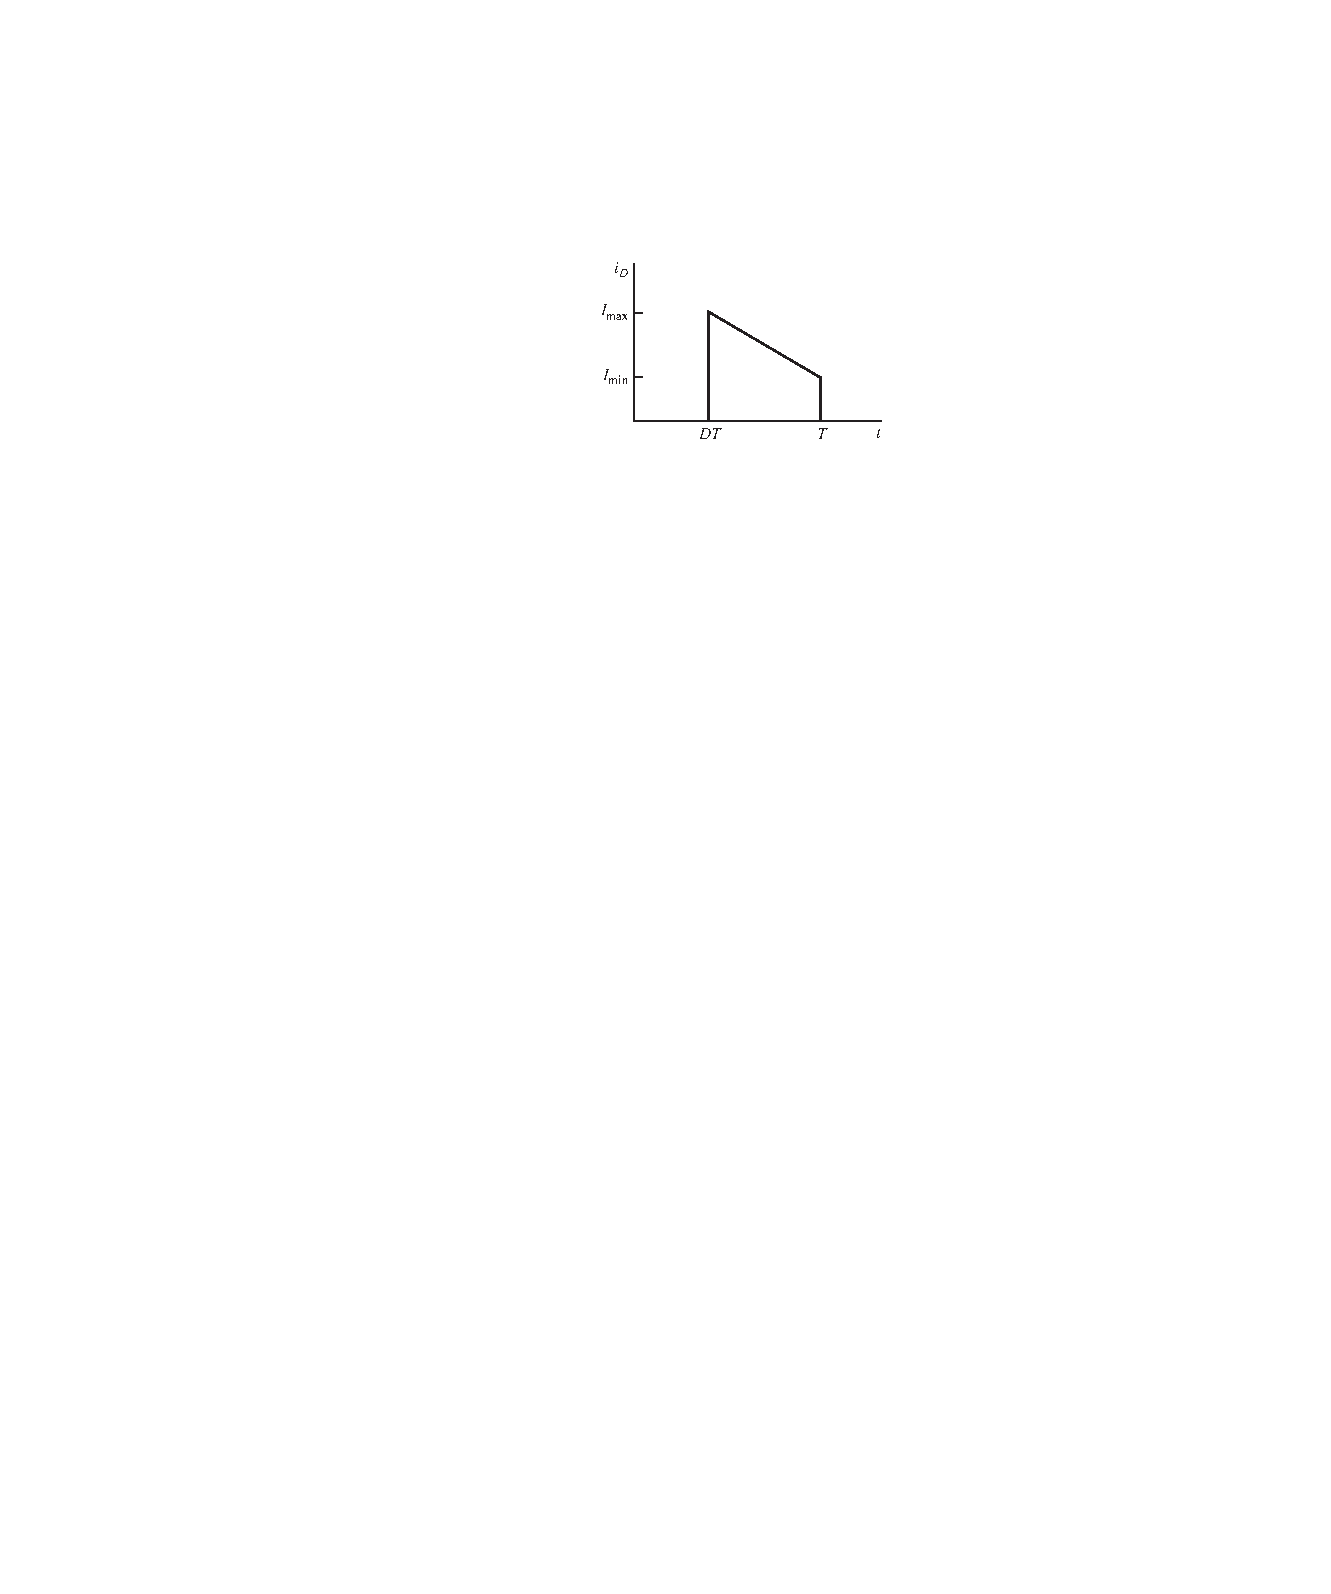
\includegraphics[width=0.38\textwidth]{Imágenes/Convertidor elevador/Corriente del diodo.pdf}}
    \hspace{10mm}
    \subfloat[Corriente por el capacitor]{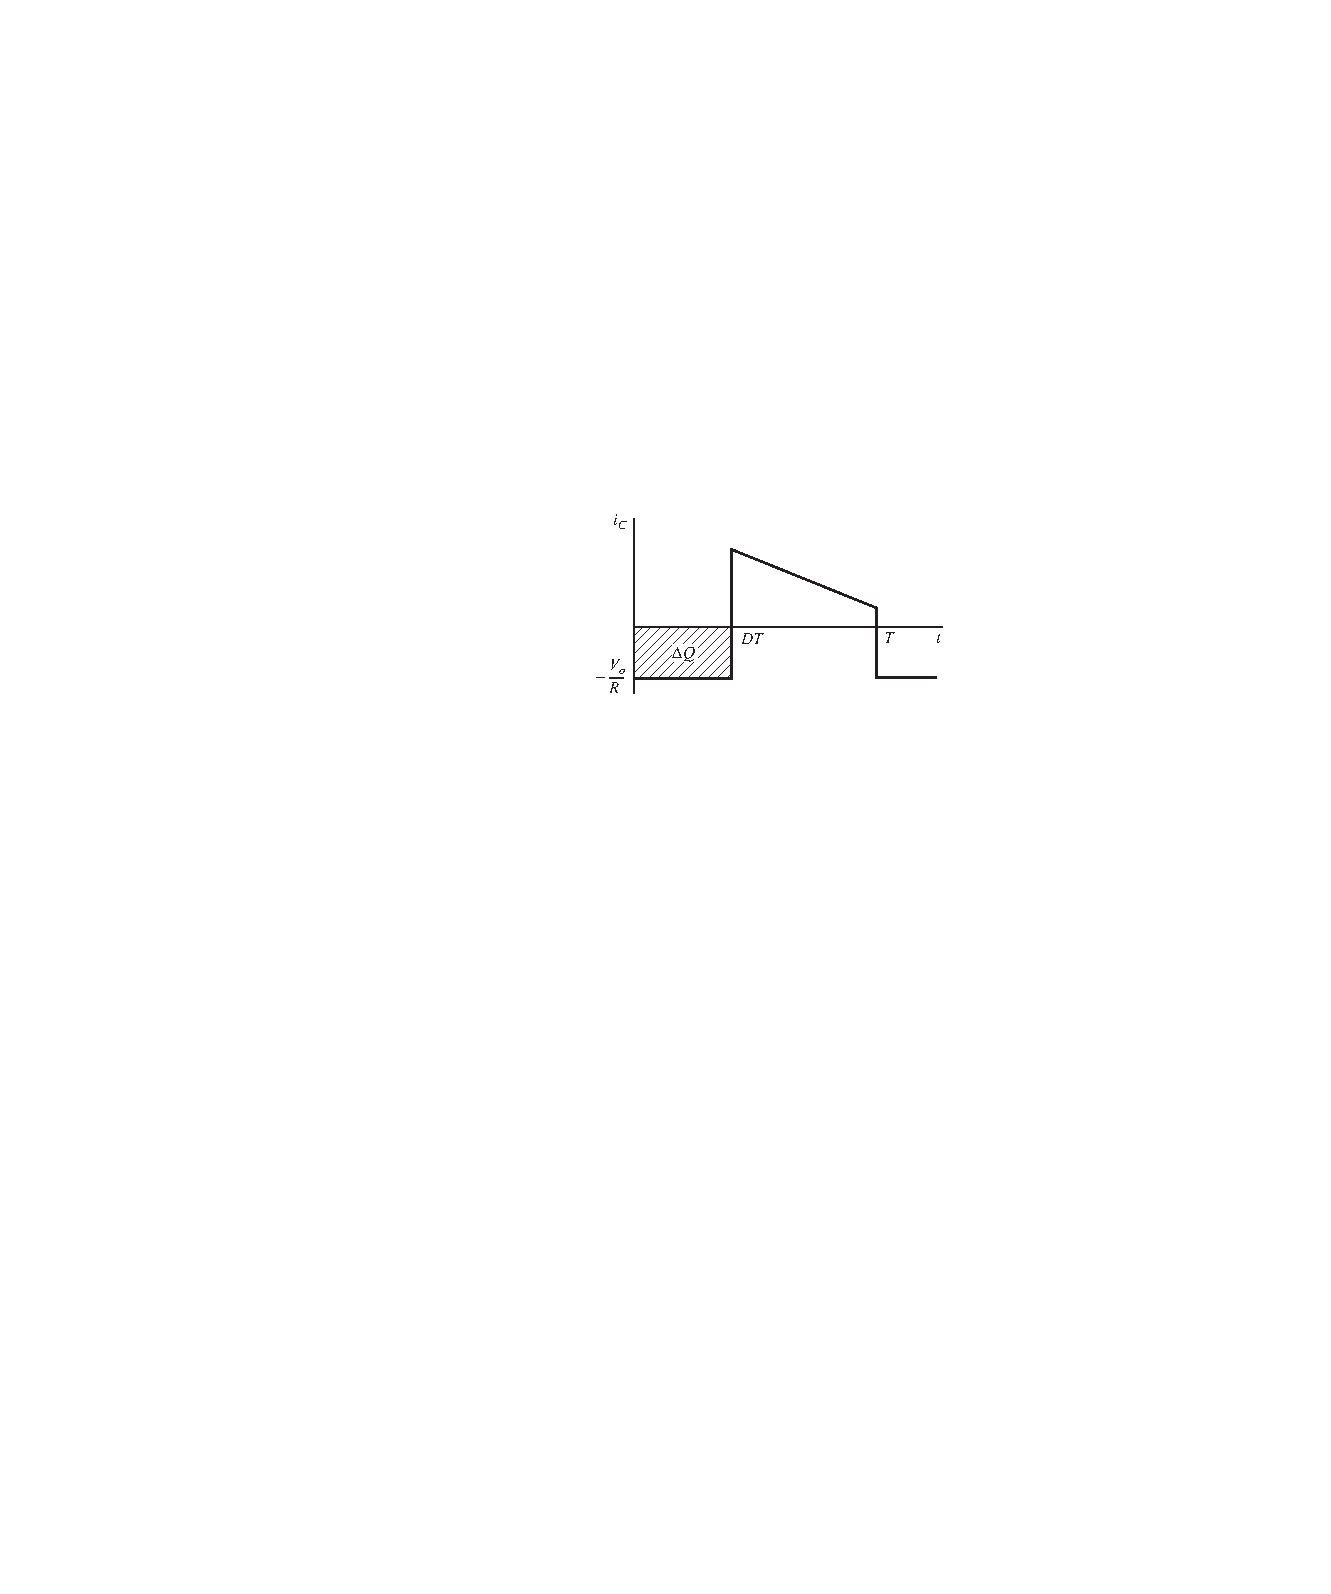
\includegraphics[width=0.38\textwidth]{Imágenes/Convertidor elevador/Corriente del capacitor.pdf}}
    \caption{Formas de onda de un convertidor elevador.}
    \label{formas-onda-elevador}
\end{figure}

\subsubsection{Análisis con la llave abierta}

Cuando la llave se abre, la corriente del inductor no puede cambiar instantáneamente, así que el diodo se polariza directamente para proveer un camino a $i_L$. Asumiendo que la tensión de salida $V_o$ es constante, la tensión que cae en el inductor es:

\begin{equation}
    v_L = V_s - V_o = L \frac{di_L}{dt} \hspace{0.6cm} \textrm{ó} \hspace{0.6cm} \frac{di_L}{dt} = \frac{V_s - V_o}{L}
\end{equation}

La derivada de $i_L$ nuevamente es una constante, entonces la corriente debe cambiar linealmente mientras la llave se encuentra abierta. La tasa de cambio en el inductor  mientras la llave se encuentre en este estado es:

\begin{equation*}
    \frac{\Delta i_L}{\Delta t} = \frac{\Delta i_L}{(1-D) T} = \frac{V_s - V_o}{L}
\end{equation*}

Resolviendo para $\Delta i_L$,

\begin{equation}
    \boxed{(\Delta i_L)_{\mathrm{abierto}} = \frac{(V_s - V_o)(1-D)T}{L}}
    \label{llave-abierta}
\end{equation}

En estado estacionario, la corriente media en el inductor debe ser cero. Utilizando las Ecuaciones~\ref{llave-cerrada}~y~\ref{llave-abierta}, 

\begin{equation*}
    \boxed{(\Delta i_L)_{\mathrm{cerrada}} + (\Delta i_L)_{\mathrm{abierto}} = 0}
\end{equation*}

\begin{equation*}
    \frac{V_s \, D \, T}{L} + \frac{(V_s - V_o)(1-D)T}{L} = 0
\end{equation*}

Y resolviendo para $V_o$,

\begin{equation*}
    V_s (D + 1 - D) - V_o (1 - D) = 0
\end{equation*}

\begin{equation}
    \boxed{V_o = \frac{V_s}{1-D}}
    \label{salida-elevador}
\end{equation}

La Ecuación \ref{salida-elevador} demuestra que si la llave siempre está abierta y $D$ es nula, la tensión de salida será la misma que la de la entrada. Si el ciclo de trabajo se va incrementando, el denominador de la Ec. \ref{salida-elevador} se va haciendo más chico, resultando en una tensión de salida cada vez más grande. Por lo tanto, se deduce que \emph{el convertidor elevador produce una tensión de salida siempre mayor o igual que la tensión de entrada}.

A su vez, según esta ecuación, si el ciclo de trabajo se aproxima a 1, la tensión de salida se hace infinita. Es necesario tener en cuenta que la deducción de la Ec. \ref{salida-elevador} fue realizada a partir de la suposición de componentes ideales. Los componentes reales, al poseer pérdidas, previenen tal evento. La Figura~\ref{formas-onda-elevador} muestra las formas de onda de corriente y tensión para el convertidor elevador.

La corriente media por el inductor es determinada al reconocer que la potencia media entregada por la fuente debe ser la misma que la potencia media absorbida por la carga.
La potencia de salida es:

\begin{equation*}
    P_o = \frac{V^2_o}{R} = V_o I_o
\end{equation*}

y la potencia de entrada es $V_s I_s = V_s I_L$. Igualando las potencias de salida y entrada y utilizando la Ecuación \ref{salida-elevador}:

\begin{equation*}
    V_s I_L = \frac{V_o^2}{R} = \frac{\left[ V_s / (1-D) \right]^2}{R} = \frac{V_s^2}{(1-D)^2} \, R
\end{equation*}

Realizando algunas substituciones y resolviendo para la corriente media del inductor, $I_L$ puede ser expresada como:

\begin{equation}
    \boxed{I_L = \frac{V_s}{(1-D)^2 R} = \frac{V_o^2}{V_s R} = \frac{V_o I_o}{V_s}}
\end{equation}

Los valores extremos de la corriente del inductor son determinados utilizando el valor medio y la tasa de cambio de la corriente de la Ec. \ref{llave-cerrada}.

\begin{equation}
    I_{max} = I_L + \frac{\Delta i_L}{2} = \frac{V_s}{(1-D)^2 R} + \frac{V_s D T}{2L}
\end{equation}

\begin{equation}
    I_{min} = I_L - \frac{\Delta i_L}{2} = \frac{V_s}{(1-D)^2 R} - \frac{V_s D T}{2L}
\end{equation}

La Ecuación \ref{salida-elevador} fue desarrollada con la suposición de que la corriente del inductor es continua y siempre positiva. Una condición de esto es que $I_{min}$ sea siempre positiva. Por lo tanto, el límite entre la corriente continua y discontinua esta dado por:

\begin{equation*}
    I_{min} = 0 = \frac{V_s}{(1-D)^2 R} - \frac{V_s D T}{2L} 
\end{equation*}

\begin{equation*}
    \frac{V_s}{(1-D)^2 R} = \frac{V_s D T}{2L} =\frac{V_s D}{2Lf} 
\end{equation*}

Despejando, se obtiene el mínimo valor de inductancia necesaria para asegurar el modo de conducción continua:

\begin{equation}
    \boxed{
    L_{min} = \frac{D(1-D)^2R}{2f}
    }
\end{equation}
\subsection{Modo de conducción discontinua}

El convertidor elevador también opera para corriente de inductor discontinua. En algunos casos, este modo de conducción es preferible por razones de control, por ejemplo para una salida regulada. La relación entre la tensión de salida y entrada origina de otras dos relaciones:

\begin{enumerate}
    \item La tensión media del inductor es cero.
    \item La corriente media del diodo es la misma que la de carga.
\end{enumerate}

Las corrientes del inductor y diodo para el modo de conducción discontinua poseen las formas de onda de la Figura \ref{formas-onda-elevador-mcd}.

\begin{figure}[hbt!]
    \centering
    \subfloat[Tensión en el inductor.]{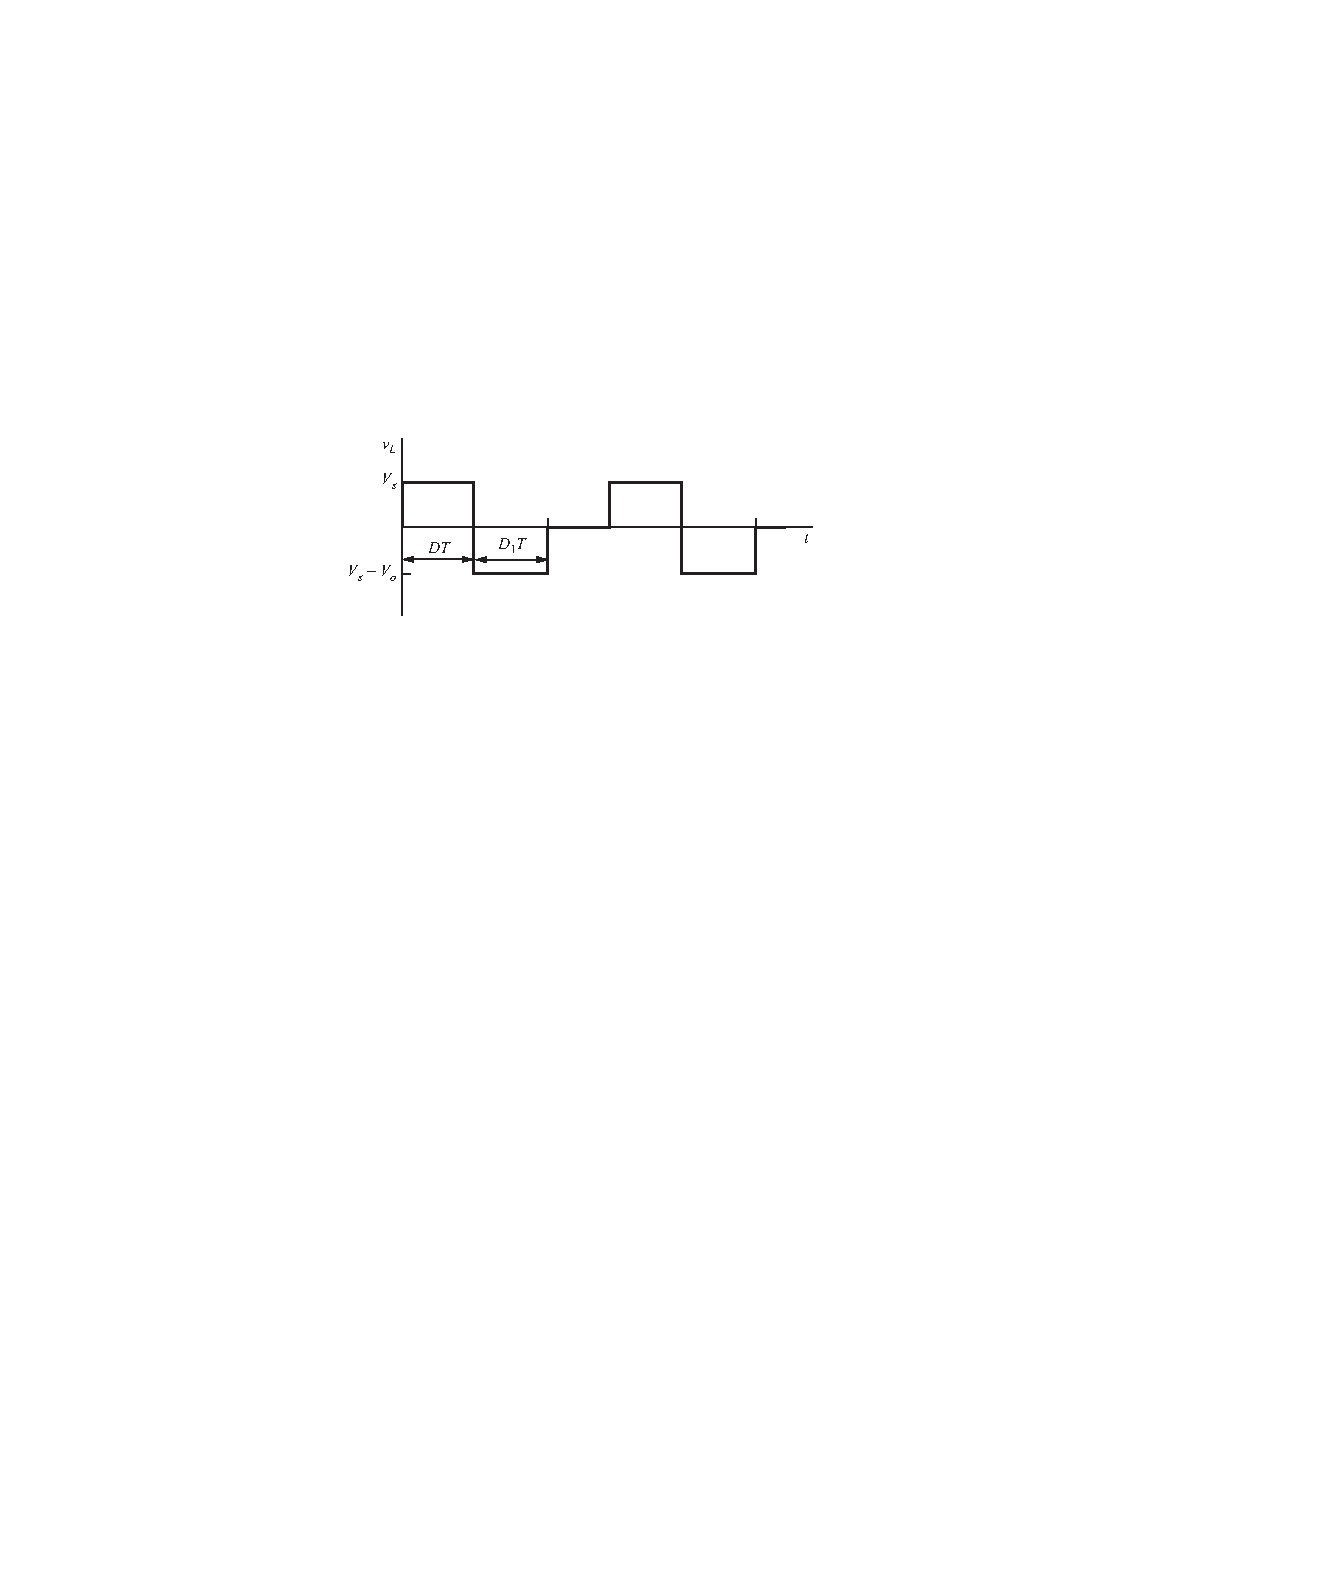
\includegraphics[width=0.38\textwidth]{Imágenes/Convertidor elevador/Modo de conducción discontinua/Tensión del inductor.pdf}}    
    \hspace{10mm}
    \subfloat[Corriente por el inductor.]{\includegraphics[width=0.38\textwidth]{Imágenes/Convertidor elevador/Modo de conducción discontinua/Corriente del inductor.pdf}}
    \hspace{10mm}
    \subfloat[Corriente por el diodo]{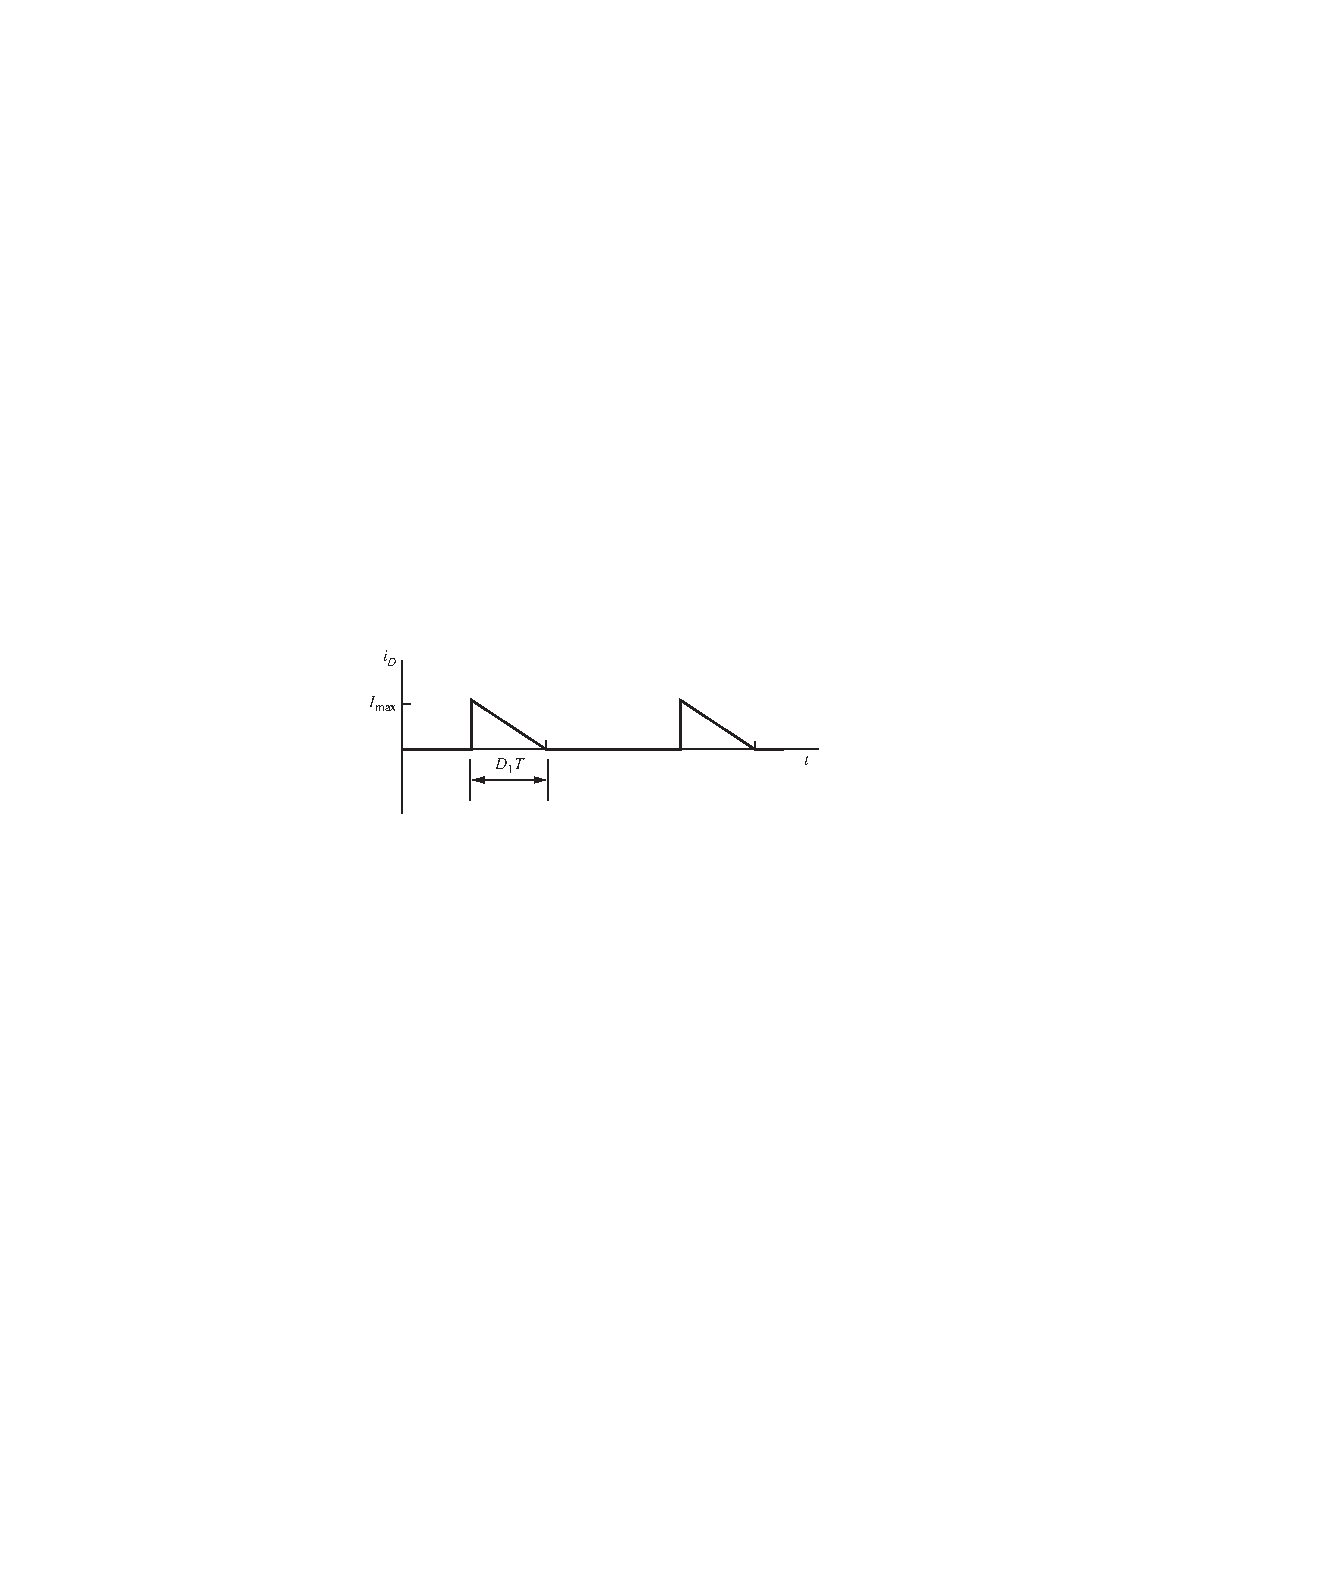
\includegraphics[width=0.38\textwidth]{Imágenes/Convertidor elevador/Modo de conducción discontinua/Corriente del diodo.pdf}}
    \caption{Formas de onda de un convertidor elevador en MCD.}
    \label{formas-onda-elevador-mcd}
\end{figure}

Cuando la llave está cerrada, la tensión a lo largo del inductor es $V_s$. Y cuando está abierta y la corriente por el inductor es positiva, su tensión es $V_s - V_o$. La corriente del inductor disminuye hasta que llega a cero, y el diodo previene que esta se haga negativa. Cuando la llave está abierta y el diodo polarizado en inversa, la corriente del inductor es nula. La tensión media que cae en el inductor es:

\begin{equation*}
    V_s D T + (V_s - V_o) D_1 T = 0
\end{equation*}

Lo que resulta en:

\begin{equation}
    V_o = V_s \left(\frac{D+D_1}{D_1}\right)
    \label{tension-salida-mcd-temp}
\end{equation}

La corriente media en el diodo (Figura \ref{formas-onda-elevador-mcd}c) es: 

\begin{equation}
    I_D = \frac{1}{T} \left(\frac{1}{2} I_{max} D_1 T\right) = \frac{1}{2} I_{max} D_1
    \label{i-diodo-temp}
\end{equation}

en donde la corriente $I_{max}$ es la misma que el cambio en la corriente del inductor cuando la llave está cerrada.

\begin{equation}
    I_{max} = \Delta i_L = \frac{V_s D T}{L}
    \label{i-inductor-max}
\end{equation}

Substituyendo la Ec. \ref{i-inductor-max} en la Ec. \ref{i-diodo-temp} e igualando con la corriente de la carga,

\begin{equation}
    I_D = \frac{1}{2} \frac{V_s D T}{L} D_1 = \frac{V_o}{R}
\end{equation}

Y despejando $D_1$,

\begin{equation}
    \boxed{D_1 = \left(\frac{V_o}{V_s}\right) \left(\frac{2L}{R D T}\right)}
\end{equation}

Substituyendo esta expresión por $D_1$ en \ref{tension-salida-mcd-temp}, resulta en la siguiente ecuación cuadrática:

\begin{equation*}
    \left(\frac{V_o}{V_s}\right)^2 - \frac{V_o}{V_s} - \frac{D^2 R T}{2L} = 0
\end{equation*}

Y finalmente resolviendo para $V_o / V_s$,

\begin{equation}
    \boxed{\frac{V_o}{V_s} = \frac{1}{2} \left(1 + \sqrt{1 + \frac{2 D^2 R T}{L}}\right)}
\end{equation}

La situación límite entre corriente continua y discontinua ocurre cuando $D_1 = 1 -D$. Otra condición límite es cuando $I_{min}$ es menor o igual a cero.

El modo de operación del convertidor depende de la combinación de los parámetros del circuito, incluyendo el ciclo de trabajo. Si este ciclo de trabajo $D$ es variado, el convertidor puede entrar y salir del modo de conducción discontinua. La Figura \ref{modo-conduccion-elevador} muestra la tensión de salida para un convertidor elevador respecto del ciclo de trabajo.

\begin{figure}[hbt!]
    \centering
    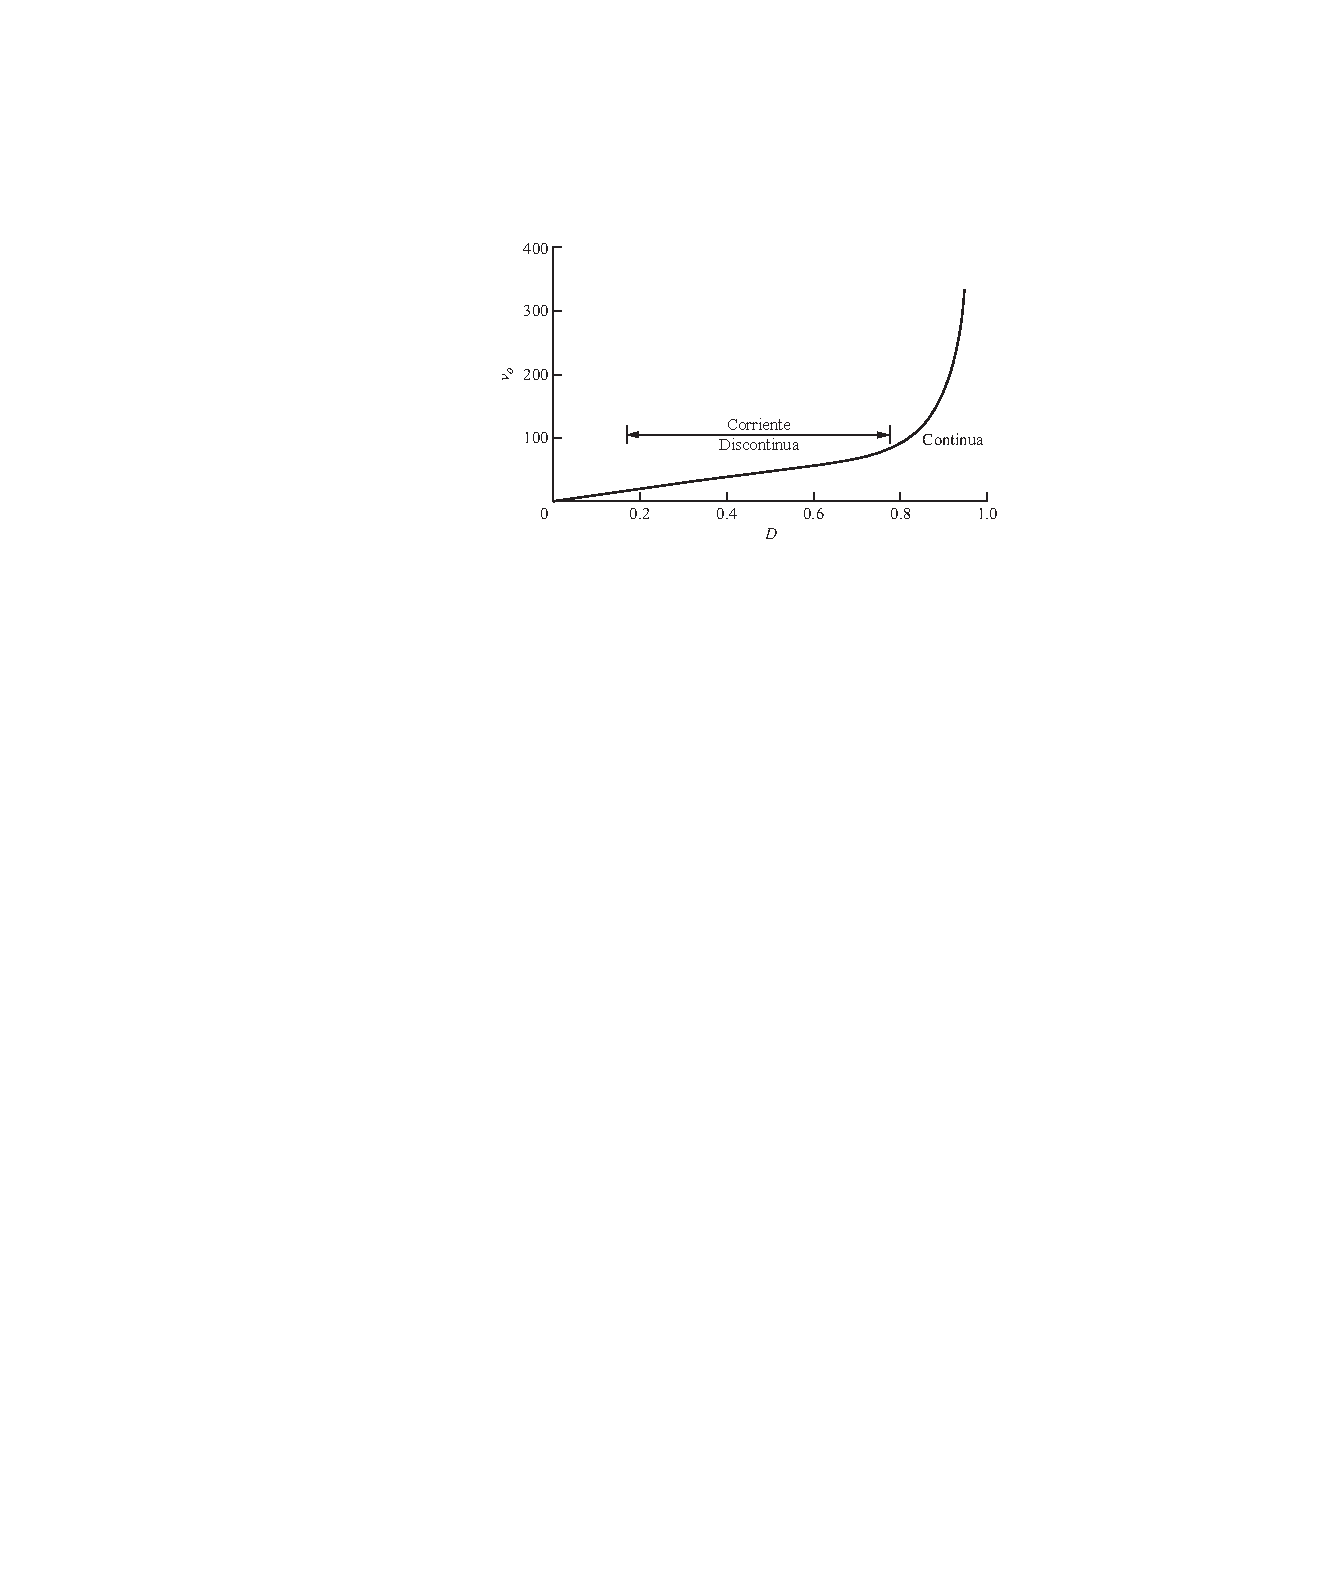
\includegraphics[width=0.55\columnwidth]{Imágenes/Convertidor elevador/Modo de conducción discontinua/Tension de salida respecto del ciclo de trabajo.pdf}
    \caption{Tensión de salida de un circuito elevador.}
    \label{modo-conduccion-elevador}
\end{figure}

\subsection{Convertidor elevador bidireccional en corriente}
\label{presentacion-convertidor}

Este tipo de convertidor es más versátil que la topología elevadora convencional, dado que tiene la capacidad de transferir energía en ambos sentidos, de la entrada a la salida y viceversa, efectuando únicamente un cambio en el sentido de la corriente.

Un convertidor elevador bidireccional en corriente se construye sustituyendo el diodo que se encuentra en la topología elevadora convencional por un transistor controlado que permita el flujo de corriente en ambas direcciones. En particular, durante el proceso de fabricación de un transistor \mbox{MOSFET} se forma una juntura p-n entre los terminales de \emph{drain} y \emph{source}, permitiendo que la corriente pueda establecerse en la dirección opuesta \emph{source-drain}. De esta forma se obtiene la bidireccionalidad de corriente a través de la llave. La topología resultante se muestra en la Figura \ref{convertidor-bidireccional}.

\begin{figure}[hbt!]
    \centering
    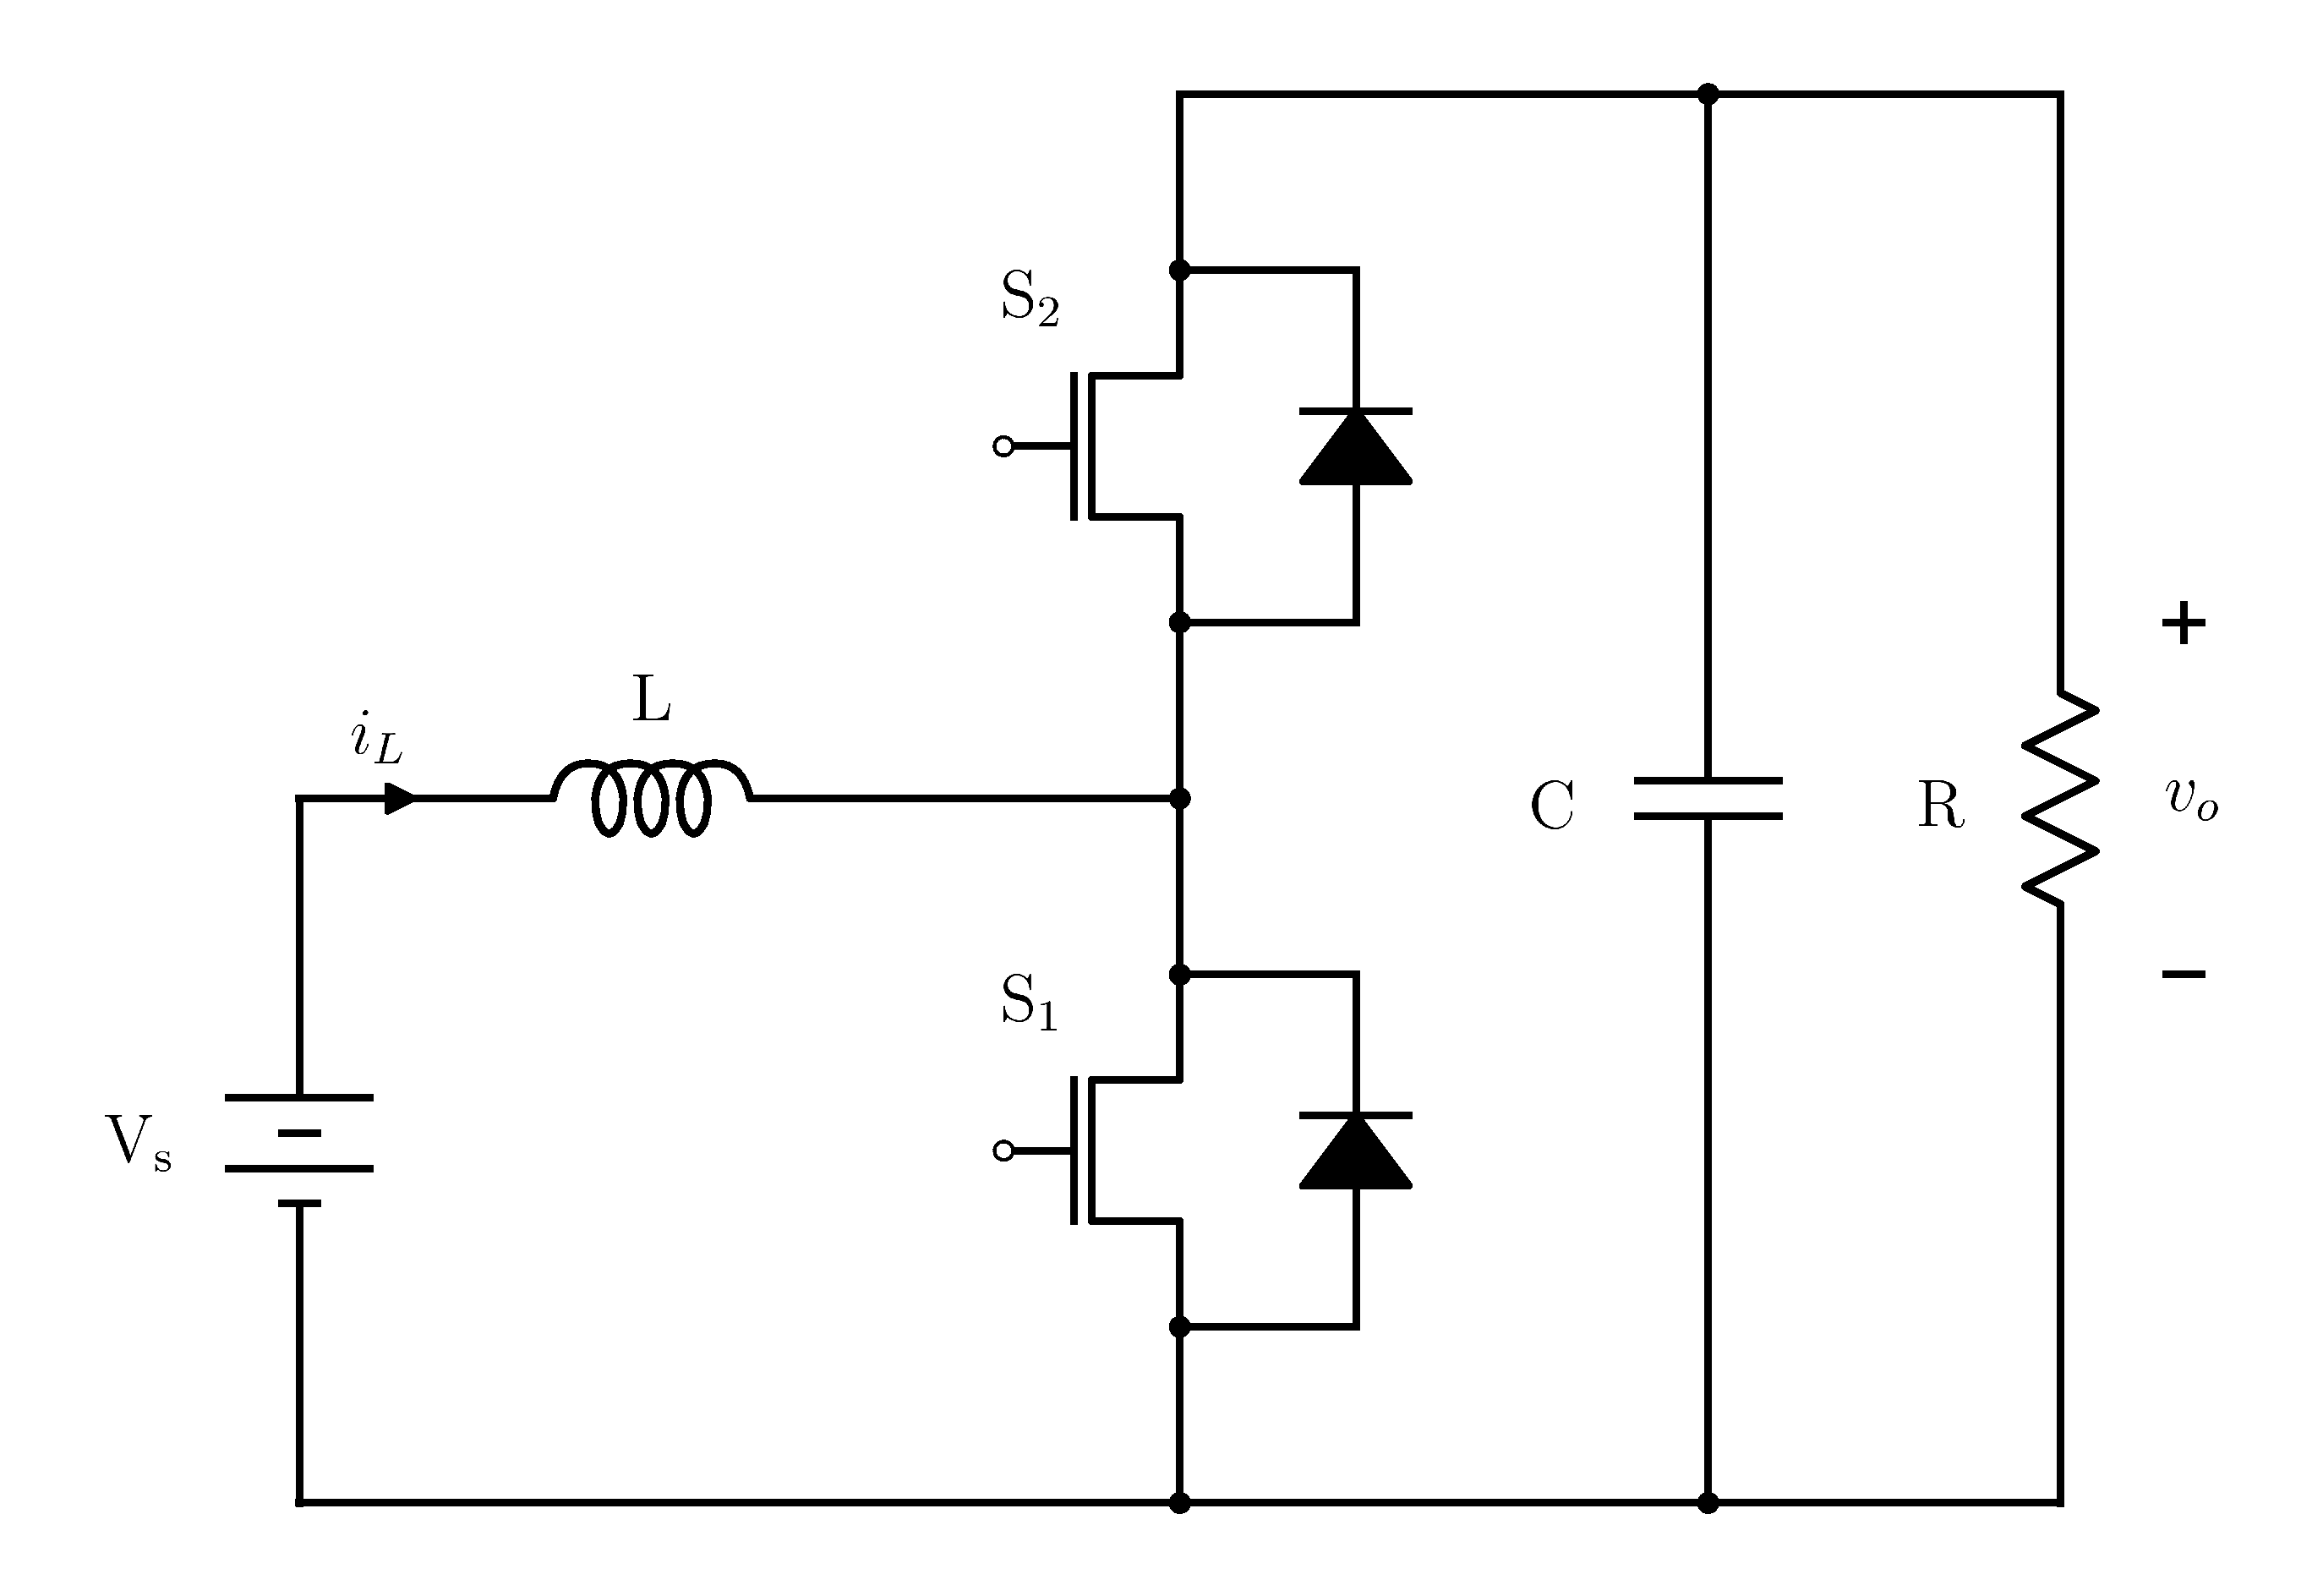
\includegraphics[width=0.40\columnwidth]{Imágenes/Diseño del control/Convertidor bidireccional de corriente.pdf}
    \caption{Convertidor elevador bidireccional en corriente.}
    \label{convertidor-bidireccional}
  \end{figure} 

Un ejemplo práctico de la aplicación de convertidores bidireccionales que facilita la comprensión de su utilidad se encuentra en el sistema de distribución de un vehículo híbrido. El vehículo tiene esencialmente 2 modos de operación:

\begin{itemize}
    \item \textbf{Modo marcha}: Para ponerse en marcha, el vehículo toma energía del banco de supercapacitores durante la aceleración y de las baterías de litio una vez estabilizada su velocidad. Durante este proceso, el convertidor transfiere energía desde los módulos de almacenamiento hacia el vehículo.
    \item \textbf{Modo regenerativo}: Una vez que el vehículo está en marcha, existe una regeneración de energía que es devuelta a los módulos de almacenamiento por parte del sistema electromecánico. Durante este proceso, el convertidor transfiere energía desde el vehículo hacia los módulos de almacenamiento.
\end{itemize}

El ejemplo anterior pone de manifiesto la gran versatilidad que se obtiene al modificar la topología elevadora clásica para lograr bidireccionalidad en el flujo de energía.

\begin{figure}[hbt!]
    \centering
    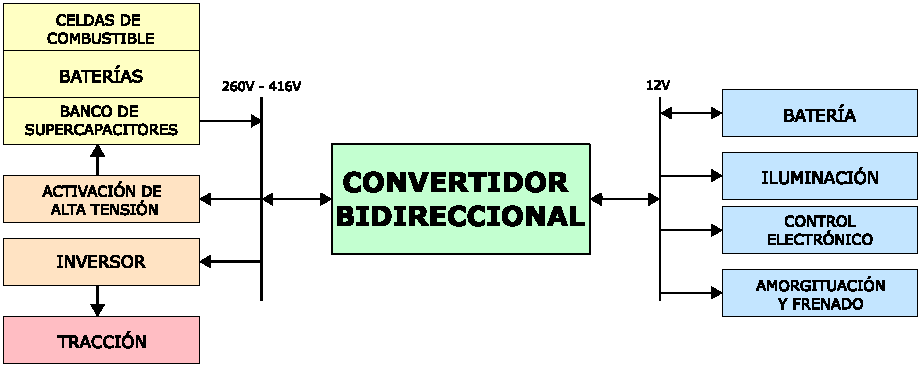
\includegraphics[width=0.75\columnwidth]{Imágenes/Convertidor elevador/Sistema eléctrico de un vehículo híbrido.pdf}
    \caption{Sistema eléctrico de un vehiculo híbrido.}
    \label{sistema-electrico-hev}
\end{figure} 

En este trabajo se utiliza un convertidor CC-CC bidireccional en corriente construido en el instituto (Figura \ref{convertidor-leici}) \cite{caravelli}. Este convertidor cuenta con una etapa de instrumentación que permite la medición de las corrientes y tensiones entrantes y salientes. En la Tablas 2.1a y 2.1b se muestran sus especificaciones técnicas.

\begin{figure}[hbt!]
    \centering
    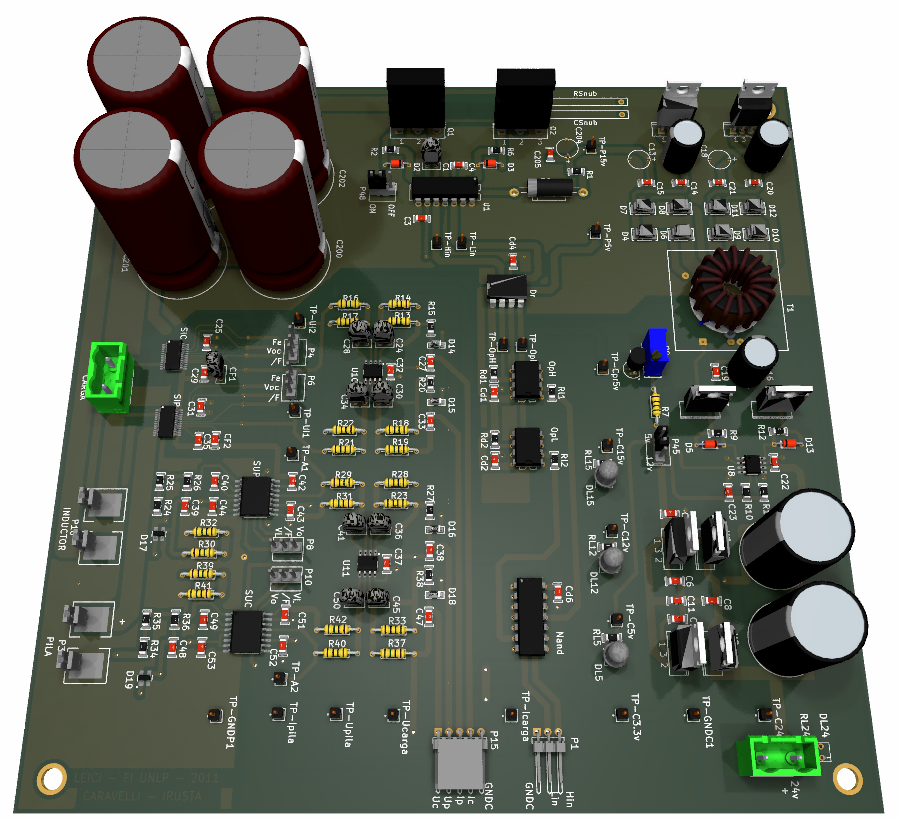
\includegraphics[width=0.52\columnwidth]{Imágenes/Convertidor elevador/Vista 3D del PCB del convertidor DC-DC.png}
    \caption{Vista 3D del convertidor DC-DC utilizado en el proyecto.}
    \label{convertidor-leici}
\end{figure} 

\begin{table}
    \centering
    \begin{tabular}{lll}
            Especificación                     & Valor & Unidad \\
            \hline
            \\
            Potencia máxima                    & 300   & W      \\
            \makecell[l]{Tensión continua \\ en la salida}      & 60    & V      \\
            \makecell[l]{Tensión nominal  \\ en la entrada}      & 20    & A      \\
            \makecell[l]{Corriente nominal \\ en la entrada}    & 15    & A      \\
            \makecell[l]{Rizado pico a pico \\ de la corriente} & 3.33  & A      \\
            \makecell[l]{Frecuencia de \\ conmutación}          & 20    & kHz     \\
            Inductancia                        & 200   & H      \\
            \makecell[l]{Corriente máxima \\ por el inductor}   & 16.67 & A      \\
            Capacitancia                       & 2200  & \SI{}{\micro\farad}
    \end{tabular}
    \label{parametros-convertidor}
    \caption{Parámetros eléctricos del convertidor CC-CC.}
\end{table}

\begin{table}
    \centering
    \begin{tabular}{lll}
        Componente          & Denominación    & Comentarios                                                    \\
        \hline\\
        \makecell[l]{Núcleo del \\ inductor} & ETD-5922 CF-138 & \makecell[l]{Permeabilidad relativa \\ $\mathrm{\mu_r}$ de 2500}                           \\
        Capacitor           & TREC            & \makecell[l]{Tensión máxima de \\ trabajo de \SI{100}{V}}                              \\
        Interruptores       & IRFP-250        & \makecell[l]{MOSFET con corriente \\ máxima de drenador de \SI{30}{A}}                \\
        Drivers             & IR2110          & \makecell[l]{Tiempo de encendido \\ y apagado de \SI{120}{\nano\second} y \SI{94}{\nano\second} \\ respectivamente} \\
        \makecell[l]{Diodo de \\ bootstrap}  & MUR 460         & \makecell[l]{Capacitancia de \SI{1}{\micro\farad} \\ con resistencia de \SI{2.2}{\ohm}}               
    \end{tabular}
    \label{componentes-convertidor}
    \caption{Componentes eléctricos del convertidor CC-CC.}

\end{table}   

\section{Resumen}

En este capítulo se ha analizado el funcionamiento de la topología de convertidor CC-CC elevador bajo distintas condiciones de conducción, y realizando una leve modificación en su estructura, se logra un tipo de convertidor CC-CC bidireccional en corriente. Finalmente, se presenta específicamente al convertidor utilizado en este proyecto.

\newpage